\chapter{입자에서 단순한 양자장으로}

이번에는 조금 다른 관점에서 단순한 양자장을 다시 구성해 보자. 양자장론으로 들어가는 길은 두 가지다. 입자에서 출발해 장이 왜 입자를 기술하는 자연스러운 언어인지 알아볼 수도 있고, 파동장에서 출발해 그 들뜸이 왜 양자 단위로 나타나는지 살펴볼 수도 있다. 두 길 모두 유용하다. 여기서는 첫 번째 길을 택한다.

보통의 양자역학은 입자 하나, 둘 또는 그 밖의 정해진 수의 입자를 기술할 수 있다. 하지만 자연은 그런 제약을 따르지 않는다. 빛이 복사를 방출하거나 흡수할 때마다 방 안의 광자 수는 변한다. 불안정 입자는 붕괴한다. 예를 들어 베타 붕괴에서는
\begin{equation}
n\longrightarrow p+e^-+\bar{\nu}_e,
\end{equation}
여러 입자 종의 개수가 동시에 변한다. 따라서 가능한 모든 점유수를 포함하고, 궁극적으로는 그 사이를 오가는 과정까지 기술할 수 있을 만큼 넓은 양자역학이 필요하다.

우선 문제를 크게 단순화하자. 비상대론적 입자 종은 하나뿐이라고 하자. 먼저 상태 공간을 확장해 임의의 입자 수를 담을 수 있게 한 다음, 다른 입자 종과 상대론, 산란, 붕괴를 논의할 것이다. 수학 자체는 특별히 어렵지 않지만 관점의 변화는 추상적이다. 표기법이 핵심 아이디어를 가리지 않도록 차근차근 살펴볼 필요가 있다.

\section{한 입자에서 출발하기}

입자 하나가 상태 \(|\psi\rangle\)에 있다고 하자. 위치 공간 파동함수는 다음과 같다.
\begin{equation}
\psi(x)=\langle x|\psi\rangle.
\label{eq:l07-wavefunction}
\end{equation}
소문자 \(\psi\)는 보통의 복소수값 함수다. 이것은 아직 양자장이 아니며, 다입자 상태 공간에 작용하는 연산자도 아니다.

보른 규칙에 따르면
\begin{equation}
\rho_\psi(x)=|\psi(x)|^2=\psi^*(x)\psi(x)
\label{eq:l07-born-density}
\end{equation}
은 위치 \(x\)에서 입자를 발견할 확률 밀도다. 정규화된 상태에서는
\begin{equation}
\int dx\,\psi^*(x)\psi(x)=1.
\label{eq:l07-one-particle-normalization}
\end{equation}
가 성립한다. 우변은 전체 확률이다. 이 문제에는 입자가 정확히 하나 있으므로, 그 값은 입자 수도 된다. 여기서는 자명한 일치지만, 나중에 유용한 실마리가 된다.

\begin{classroomqa}
\lecturetimestamp{00:09:13}
\audiencequestion{확률 밀도가 왜 \(\psi^*(x)\psi(x)\)의 형태여야 하나요?}
\lecturerresponse{그것이 양자역학의 공리 가운데 하나인 보른 규칙입니다. 위치 측정 결과 \(x\)에 대응하는 진폭은 \(\langle x|\psi\rangle\)이고, 확률 밀도는 그 절댓값의 제곱입니다. 이것은 뒤에서 사용할 장의 구성으로부터 유도되는 것이 아닙니다.}
\end{classroomqa}

\section{모드, 직교성, 완비성}

한 입자 힐베르트 공간에는 유용한 기저가 여럿 있다. 위치 고유상태들이 한 기저를 이룬다. 적절한 조건 아래 에르미트 연산자의 고유상태들도 다른 기저를 이룬다. 퇴화와 연속 스펙트럼의 경우에는 통상적인 주의가 필요하다. 곧 에너지가 중요해지므로, 완비 정규직교 한 입자 에너지 고유상태 집합을 택하자.
\begin{equation}
|1\rangle,\ |2\rangle,\ldots,
\qquad
\psi_i(x)=\langle x|i\rangle.
\end{equation}

상자 속 입자를 생각하면 첨자 \(i\)의 의미가 구체적으로 드러난다. 바닥 상태 파동함수에는 내부 마디가 없고, 그다음 상태에는 마디가 하나 있으며, 더 높은 상태일수록 더 빠르게 진동한다. 이상적인 무한 사각 우물에서는 이 파동함수들이 사실상 사인파다.

\begin{figure}[htbp]
\centering
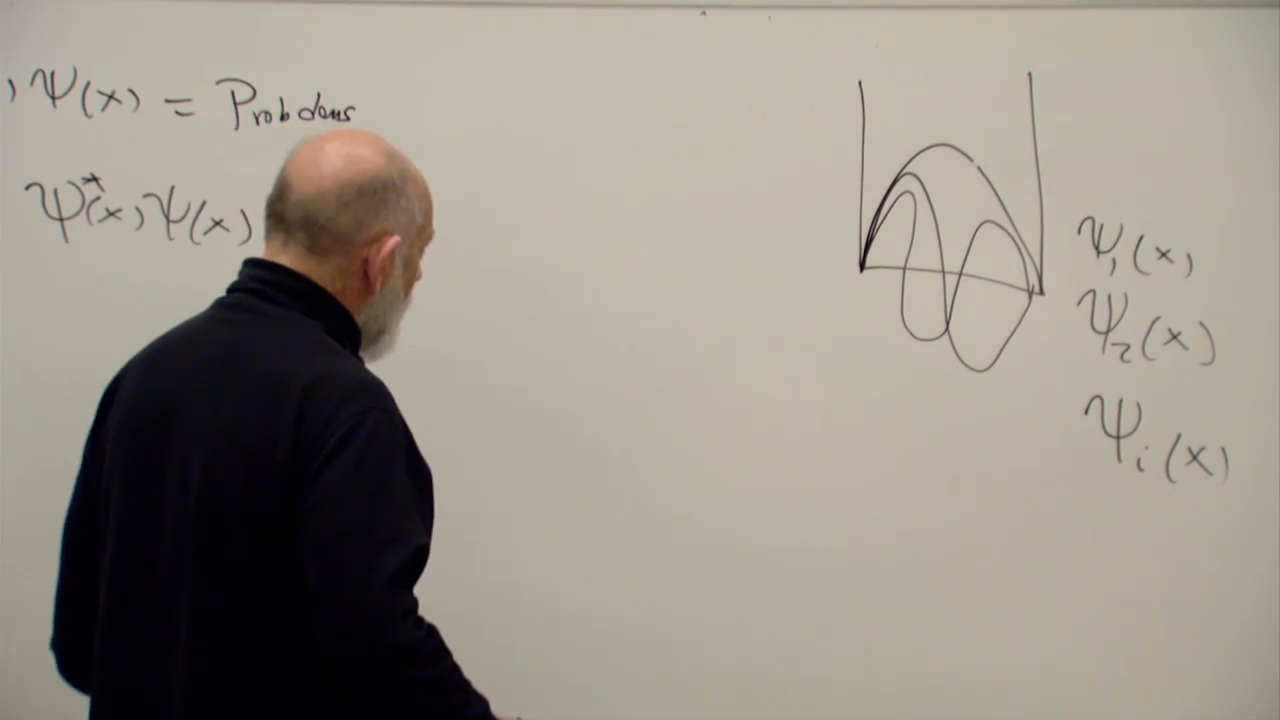
\includegraphics[width=0.94\linewidth]{lecture_07_frame_01.png}
\caption{강의 칠판에 그린 상자 모드. 왼쪽에는 한 입자 보른 밀도와 정규화 식의 일부가 남아 있고, 오른쪽 우물에는 \(\psi_1(x)\), \(\psi_2(x)\) 및 일반적인 표기 \(\psi_i(x)\)가 나타나 있다.}
\lectureframe{00:08:25}
\end{figure}

실시간 칠판 화면에 가려진 부분을 제외하면 같은 모드 구조를 다음처럼 분리해 볼 수 있다.
\begin{figure}[htbp]
\centering
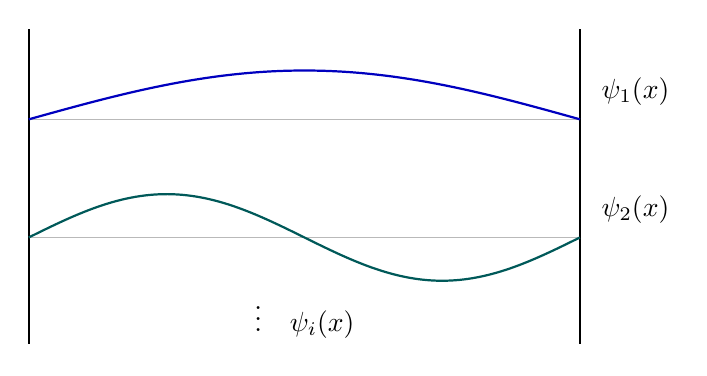
\begin{tikzpicture}[x=1cm,y=1cm]
  \draw[thick] (0,0) -- (0,4.0);
  \draw[thick] (7,0) -- (7,4.0);
  \draw[gray!55] (0,2.85) -- (7,2.85);
  \draw[gray!55] (0,1.35) -- (7,1.35);
  \draw[blue!75!black,thick,domain=0:7,samples=120]
    plot (\x,{2.85+0.62*sin(180*\x/7)});
  \draw[teal!70!black,thick,domain=0:7,samples=120]
    plot (\x,{1.35+0.55*sin(360*\x/7)});
  \node[right] at (7.15,3.20) {$\psi_1(x)$};
  \node[right] at (7.15,1.70) {$\psi_2(x)$};
  \node at (3.5,0.38) {$\vdots\quad\psi_i(x)$};
\end{tikzpicture}
\caption{상자 스케치를 정성적으로 깔끔하게 다시 그린 그림. 두 파동함수의 수직 위치를 달리한 것은 표시를 위한 것일 뿐이다.}
\end{figure}

정규직교성은 다음과 같다.
\begin{equation}
\int dx\,\psi_i^*(x)\psi_j(x)=\delta_{ij}.
\label{eq:l07-orthonormality}
\end{equation}
\(i=j\)일 때 상태는 정규화되어 적분값은 하나다. \(i\ne j\)일 때 두 상태는 서로 직교하며 적분값은 영이 된다.

완비성도 마찬가지로 중요한 명제다.
\begin{equation}
\sum_i |i\rangle\langle i|=\mathbf 1.
\label{eq:l07-resolution}
\end{equation}
각 \(|i\rangle\langle i|\)는 한 기저 방향으로의 사영이고, 완비 기저 전체에 대한 합은 항등 연산자다. 임의의 벡터에 작용시키면 그 벡터를 성분들로 분해한 뒤 다시 합친다.

이제 위치 상태 두 개 사이에 식~\eqref{eq:l07-resolution}을 끼워 넣자.
\begin{align}
\langle y|x\rangle
&=\sum_i\langle y|i\rangle\langle i|x\rangle \\
&=\sum_i\psi_i(y)\psi_i^*(x) \\
&=\delta(y-x).
\label{eq:l07-position-completeness}
\end{align}
복소켤레 표시는 브라-켓 순서가 \(\langle i|x\rangle\)인 인자에 붙는다. \(x\)와 \(y\)의 순서를 바꾸면 복소켤레를 취한 동등한 형태를 얻는다. 따라서 완비 정규직교 기저라면 어느 것이든 델타 함수의 표현을 제공한다. 사인 함수, 코사인 함수, 조화 진동자 파동함수, 에너지 고유함수가 모두 같은 역할을 한다.

\begin{classroomqa}
\lecturetimestamp{00:13:43}
\audiencequestion{완비성 합에서 두 번째 파동함수에도 복소켤레를 붙여야 하나요?}
\lecturerresponse{네. 순서가 \(\langle y|i\rangle\langle i|x\rangle\)이면 인자들은 \(\psi_i(y)\psi_i^*(x)\)입니다. 브라-켓 순서를 눈에 보이게 유지하면 복소켤레 표시를 추측하거나 잘못 붙일 일이 없습니다.}
\end{classroomqa}

이것이 앞으로 필요한 한 입자 수학이다. 이제 상태 공간을 바꾸자.

\section{더 큰 상태 공간으로서의 포크 공간}

동일한 입자가 여러 개 있을 때는 각 한 입자 모드에 몇 개의 입자가 점유되어 있는지를 기록하는 기저가 편리하다.
\begin{equation}
|n_1,n_2,n_3,\ldots\rangle.
\label{eq:l07-fock-basis}
\end{equation}
정수 \(n_i\)는 모드 \(i\)의 점유수다. 이 켓은 한 입자 상태를 그럴듯한 표기로 쓴 것이 아니다. 입자가 없는 부문, 모든 한 입자 상태, 모든 두 입자 상태 등을 포함하는 더 큰 힐베르트 공간에 속한다. 이 더 큰 공간을 포크 공간이라 한다.

점유수를 바꾸기 위해 각 모드에 대해 생성 연산자와 소멸 연산자를 도입하자.
\begin{equation}
a_i^\dagger,\qquad a_i.
\end{equation}
첫 번째 연산자는 모드 \(i\)에 입자 하나를 더하고, 두 번째 연산자는 하나를 제거한다. 여기서 조화 진동자라는 표현은 점유수를 올리고 내리는 데 필요한 대수 구조를 제공하는 계산상의 도구다. 실제로 진동하는 용수철이 존재할 필요는 없다.

모드 수 연산자는 다음과 같다.
\begin{equation}
\begin{aligned}
N_i&=a_i^\dagger a_i,\\
N_i|n_1,\ldots,n_i,\ldots\rangle
&=n_i|n_1,\ldots,n_i,\ldots\rangle.
\end{aligned}
\end{equation}
진공 상태는
\begin{equation}
|0\rangle\equiv|0,0,0,\ldots\rangle,
\qquad
a_i|0\rangle=0
\quad\text{for every }i.
\label{eq:l07-vacuum}
\end{equation}
이다. 따라서 모드 \(i\)의 한 입자 상태는
\begin{equation}
|i\rangle=a_i^\dagger|0\rangle.
\label{eq:l07-mode-created}
\end{equation}
가 된다. 같은 기호 \(|i\rangle\)는 이제 한 입자 기저 벡터로도, 포크 공간의 한 입자 부문에 포함된 그 벡터로도 해석할 수 있다. 그 포함 관계를 나타내는 식은 ~\eqref{eq:l07-mode-created}이고, 어느 공간을 논하는지는 주변 문맥으로 판단한다.

\section{모드들을 하나의 장으로 묶기}

소멸장과 생성장을 다음과 같이 정의하자.
\begin{equation}
\Psi(x)=\sum_i \psi_i(x)a_i,
\qquad
\Psi^\dagger(x)=\sum_i \psi_i^*(x)a_i^\dagger.
\label{eq:l07-field-expansion}
\end{equation}
대문자 표기가 중요하다. 소문자 함수 \(\psi_i(x)\)는 복소수이고, 대문자 \(\Psi(x)\)는 포크 공간에 작용하는 연산자다. 각 공간점 \(x\)에서 식~\eqref{eq:l07-field-expansion}은 모드 연산자들의 서로 다른 선형 결합을 준다. 이것이 위치의 연산자값 함수라는 말의 뜻이다.

자유 입자에서는 모드 함수가 평면파 \(e^{ikx}\)일 수 있다. 그러면 식~\eqref{eq:l07-field-expansion}은 푸리에 전개와 같지만 푸리에 계수가 수가 아니라 연산자다. 옛 용어에서는 보통의 복소수를 \(c\)수, 양자 연산자를 \(q\)수라 부른다. 모드 함수는 \(c\)수이므로 모든 것과 가환한다. 연산자 성질은 \(a_i\)와 \(a_i^\dagger\)가 지닌다.

\(\Psi\)와 \(\Psi^\dagger\)는 어느 쪽도 에르미트 연산자가 아니다. 두 연산자는 서로의 수반이다. 다음 두 조합은
\begin{equation}
\Psi+\Psi^\dagger,
\qquad
i(\Psi^\dagger-\Psi)
\label{eq:l07-hermitian-combinations}
\end{equation}
에르미트 연산자이므로 관측량을 나타낼 수 있다. 그러나 지금은 장을 국소적으로 입자를 생성하고 소멸시키며 그 수를 세는 도구로 사용하는 것이 가장 유용하다.

\begin{classroomqa}
\lecturetimestamp{00:21:05}
\audiencequestion{연산자가 \(x\)에 의존한다는 것은 무슨 뜻인가요?}
\lecturerresponse{각 \(x\) 값이 서로 다른 연산자를 지정한다는 뜻입니다. 공간 의존성은 보통의 모드 함수에 들어 있고, 그에 따라 만들어지는 각 선형 결합은 동일한 포크 공간에 작용합니다.}
\end{classroomqa}

\section{생성장이 하는 일}

정의는 그것이 무엇을 하는지 물어볼 때 유용해진다. 한 입자 부문의 위치 고유상태에서 시작해 항등 연산자의 분해를 끼워 넣자.
\begin{align}
|x\rangle
&=\sum_i |i\rangle\langle i|x\rangle \\
&=\sum_i a_i^\dagger|0\rangle\,\psi_i^*(x) \\
&=\Psi^\dagger(x)|0\rangle.
\label{eq:l07-local-creation}
\end{align}
따라서 \(a_i^\dagger\)은 정해진 모드 \(i\)에 입자를 생성하고, \(\Psi^\dagger(x)\)는 위치 \(x\)에 국소화된 입자를 생성한다. 이상화된 위치 기저에서 이 국소화는 분포의 의미로 이해해야 한다. 실제로 입자를 준비할 때는 좁은 파동묶음을 쓰겠지만, 대수적인 의미는 같다.

\begin{classroomqa}
\lecturetimestamp{00:24:48}
\audiencequestion{\(\sum_i|i\rangle\langle i|\)은 사영 연산자인가요?}
\lecturerresponse{각 항은 한 기저 상태로의 사영입니다. 완비 기저 전체에 대한 합은 항등 연산자 자체이며, 항등 연산자의 분해라 부릅니다. 이를 끼워 넣어도 상태는 변하지 않지만, 선택한 기저에서 그 상태의 성분을 드러내게 됩니다.}
\end{classroomqa}

식~\eqref{eq:l07-local-creation}은 장에 대한 첫 번째 직접적인 입자 해석을 보여 준다. 추상적인 연산자에 공간 표지만 덧붙인 것이 아니다. 그 공간점에 입자를 만드는 작용을 구성했다.

\begin{classroomqa}
\lecturetimestamp{00:28:20}
\audiencequestion{위치 공간 생성장에는 별표와 대거 중 무엇을 붙여야 하나요?}
\lecturerresponse{연산자의 수반에는 대거를 씁니다. 별표는 보통의 파동함수 \(\psi_i(x)\)의 복소켤레에 쓰고, 대거는 \(a_i^\dagger\)와 \(\Psi^\dagger(x)\)에 붙입니다.}
\end{classroomqa}

\begin{classroomqa}
\lecturetimestamp{00:28:36}
\audiencequestion{모드 전개식에서 생성 연산자를 파동함수 너머로 옮겨도 되나요?}
\lecturerresponse{네. \(\psi_i(x)\)는 \(c\)수이므로 모든 연산자와 가환합니다. \(a_i\)와 \(a_j^\dagger\)처럼 서로 가환하지 않는 연산자의 순서를 바꿀 때만 주의하면 됩니다.}
\end{classroomqa}

\section{확률 밀도에서 입자 밀도로}

이제 장을 살펴보자. 가장 먼저 떠오르는 식은
\begin{equation}
\int dx\,\Psi^\dagger(x)\Psi(x).
\end{equation}
이다. 한 입자 정규화 적분과 비슷해 보이지만, 이제 인자들은 연산자다. 순서를 바꾸지 않고 모드 전개를 대입하자.
\begin{align}
\int dx\,\Psi^\dagger(x)\Psi(x)
&=\int dx
\left(\sum_i a_i^\dagger\psi_i^*(x)\right)\\
&\qquad\times\left(\sum_j a_j\psi_j(x)\right) \\
&=\sum_{i,j}a_i^\dagger a_j
\int dx\,\psi_i^*(x)\psi_j(x) \\
&=\sum_{i,j}a_i^\dagger a_j\,\delta_{ij} \\
&=\sum_i a_i^\dagger a_i.
\label{eq:l07-number-derivation}
\end{align}
따라서 전체 입자 수 연산자는
\begin{equation}
N=\sum_i N_i
=\int dx\,\Psi^\dagger(x)\Psi(x).
\label{eq:l07-total-number}
\end{equation}
이다. 여기서 다루는 상태에서는 유한한 에너지의 들뜸이 충분히 높은 모드 에너지에서 점유수가 감소하므로, 가능한 모드 목록은 무한해도 이 전체 입자 수는 보통 유한하다.

적분 안의 함수는 국소 입자 밀도 연산자다.
\begin{equation}
n(x)=\Psi^\dagger(x)\Psi(x).
\label{eq:l07-density}
\end{equation}
엄밀히 말해 수학적 점 하나에서 밀도를 측정할 수는 없다. 작은 영역 \(R\)에 대해서는
\begin{equation}
N_R=\int_R dx\,n(x),
\label{eq:l07-regional-number}
\end{equation}
을 측정하는데, 이는 그 영역 안의 입자 수다. 다른 양자 관측량과 마찬가지로 \(N_R\)도 임의의 상태에서 정해진 값을 가져야 하는 것은 아니다. 같은 준비를 반복해도 측정 결과가 달라질 수 있다.

\begin{classroomqa}
\lecturetimestamp{00:36:27}
\audiencequestion{\(\Psi^\dagger(x)\Psi(x)\)은 다입자 확률 밀도인가요?}
\lecturerresponse{직접적인 의미는 입자 밀도입니다. 다입자 확률 진폭은 일반적으로 모든 입자 좌표에 의존합니다. 반면 이 국소 쌍선형식은 작은 영역에 대해 적분하면 그 영역 안의 입자 수를 셉니다.}
\end{classroomqa}

\begin{classroomqa}
\lecturetimestamp{00:38:28}
\audiencequestion{연산자 \(a_i\)와 \(a_i^\dagger\)는 한 입자 파동함수가 아니라 상태 벡터에만 작용하나요?}
\lecturerresponse{네. 이 연산자들은 \(|n_1,n_2,\ldots\rangle\)와 같은 포크 공간 상태에 작용합니다. 이 연산자들에 곱해지는 한 입자 모드 함수는 보통의 수이며, 사다리 연산자가 작용하는 대상이 아닙니다.}
\end{classroomqa}

점유수 켓은 기저를 이루지만 가장 일반적인 상태는 아니다. 이들을 중첩할 수 있으며, 총입자 수가 같더라도 그 입자들이 모드 사이에 다르게 분포하는 상태들을 중첩할 수도 있다. 광자처럼 전기적으로 중성인 종에서는 총입자 수가 서로 다른 상태도 중첩할 수 있다. 식~\eqref{eq:l07-regional-number}의 연산자는 이런 모든 상태에서 같은 조작적 의미를 유지한다.

\begin{classroomqa}
\lecturetimestamp{00:40:01}
\audiencequestion{입자 밀도를 전체 입자 수로 나누면 위치 \(x\)에서 입자를 발견할 확률 밀도가 되나요?}
\lecturerresponse{입자 수 \(N\)가 고정된 큰 개체수 상황에서는 \(N_R/N\)가 상대도수이므로 대개 한 입자 확률과 잘 맞습니다. 그렇다고 한 번의 측정 결과를 확률과 동일시하는 연산자 항등식이 되는 것은 아닙니다. 독립 입자 그림에서는 측정된 입자 수가 보통 \(\sqrt N\) 정도의 크기로 요동합니다. 확률이 낮기는 해도 예외적인 한 번의 결과가 확률에서 크게 벗어날 수 있습니다.}
\end{classroomqa}

\begin{classroomqa}
\lecturetimestamp{00:42:25}
\audiencequestion{전자 하나가 있는 상태와 전자가 없는 상태를 중첩하면 전하 보존은 어떻게 되나요?}
\lecturerresponse{그런 중첩은 전기 전하가 고정된 닫힌 부문에서 사용하는 중첩이 아닙니다. 총전하가 같은 서로 다른 분포는 중첩할 수 있습니다. 광자는 전하를 띠지 않으므로 광자 수가 다른 부문을 중첩해도 그런 문제는 없습니다. 전자 수와 양전자 수도 순전하가 고정된 채 함께 변할 수 있습니다.}
\end{classroomqa}

\section{독립 입자의 에너지}

다음 관측량은 에너지다. 우선 서로 상호작용하지 않는 입자들로 한정하자. 희박한 계에서는 이것이 흔히 좋은 근사다. 광자도 원리적으로는 고차 과정에서 상호작용하지만, 보통의 실험실 복사는 충분히 희박해서 독립 입자 기술이 매우 정확하다.

\(\omega_i\)를 모드 \(i\)에 있는 입자 하나의 에너지라 하고, \(\hbar=1\)라고 하자. 모드는 한 입자 상태 하나를 뜻한다. 그러면 전체 해밀토니안은
\begin{equation}
H=\sum_i\omega_i N_i
=\sum_i\omega_i a_i^\dagger a_i.
\label{eq:l07-mode-hamiltonian}
\end{equation}
이다. 각 점유 모드는 입자 하나당 한 번씩 그 입자 에너지를 기여한다.

\begin{classroomqa}
\lecturetimestamp{00:48:16}
\audiencequestion{\(\omega_i\)은 위치의 함수인가요?}
\lecturerresponse{아닙니다. 이것은 모드 \(i\)에 대응하는 에너지 고윳값입니다. 함수 \(\psi_i(x)\)는 위치에 의존하고, \(\omega_i\)는 선택된 에너지 준위에 따라 정해집니다.}
\end{classroomqa}

값 \(\omega_i\)는 한 입자 시간 독립 슈뢰딩거 방정식으로 결정된다. 다음을 정의하자.
\begin{equation}
h=-\frac{\nabla^2}{2m}+V(x).
\label{eq:l07-one-particle-h}
\end{equation}
그러면
\begin{equation}
h\psi_i(x)=\omega_i\psi_i(x).
\label{eq:l07-schrodinger-eigenvalue}
\end{equation}
이다. 일차원에서 운동량 연산자는 \(p=-i\partial_x\)이므로, \(p^2/(2m)\)는 \(-\partial_x^2/(2m)\)가 된다. 삼차원에서는 세 개의 이계 도함수가 합쳐져 \(-\nabla^2/(2m)\)가 된다.

\begin{figure}[htbp]
\centering
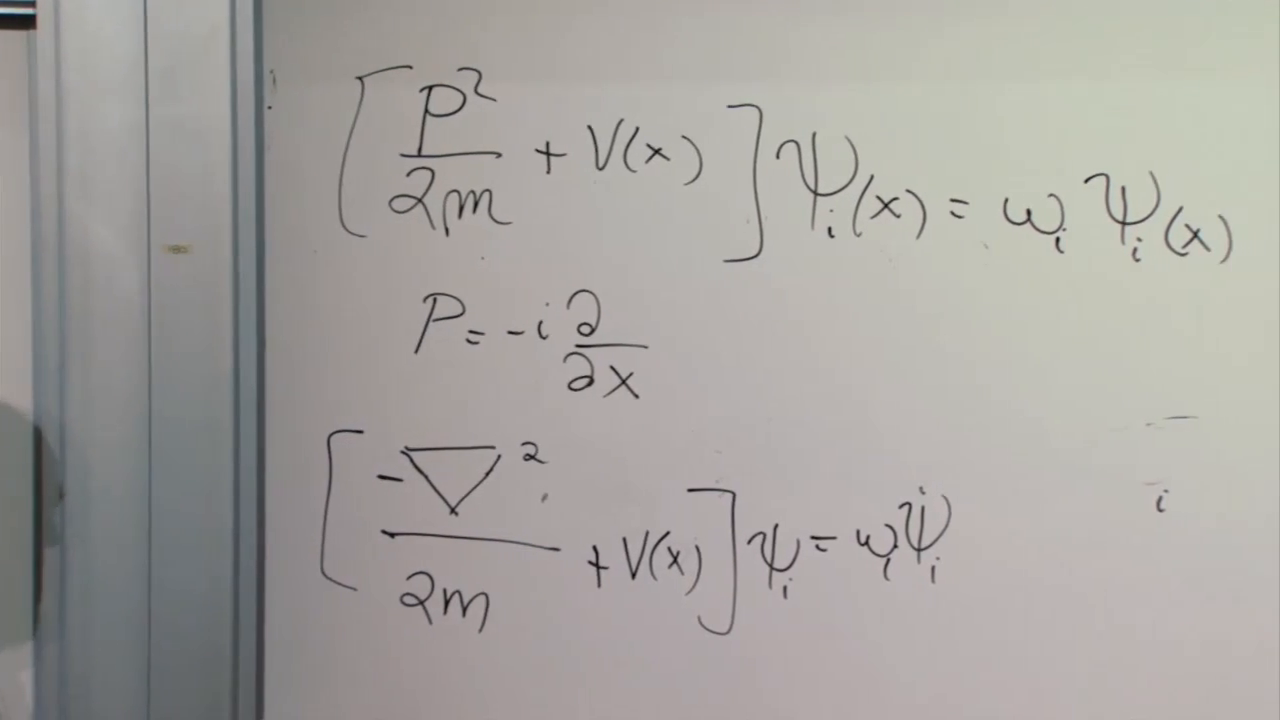
\includegraphics[width=0.94\linewidth]{lecture_07_frame_02.png}
\caption{\(p^2/(2m)+V(x)\)에서 한 입자 슈뢰딩거 고유값 방정식의 미분형으로 넘어가는 칠판 장면. 식~\eqref{eq:l07-schrodinger-eigenvalue}은 이를 깔끔하게 다시 구성한 것이다.}
\lectureframe{00:54:10}
\end{figure}

임의의 정규화된 한 입자 파동함수에 대해 잘 알려진 기댓값은 다음과 같다.
\begin{equation}
\langle h\rangle_\psi
=\int dx\,\psi^*(x)h\psi(x).
\label{eq:l07-one-particle-energy-expectation}
\end{equation}
소문자 파동함수를 연산자값 장으로 바꾸면 다입자 공식도 얻을 수 있을 듯하다. 아직 증명된 것은 아니며, 이제 타당성을 확인할 추측이다.
\begin{equation}
H=\int dx\,\Psi^\dagger(x)h\Psi(x).
\label{eq:l07-field-hamiltonian}
\end{equation}

\section{답을 먼저 쓰고 증명하기}

제안한 해밀토니안에 식~\eqref{eq:l07-field-expansion}을 대입하자.
\begin{align}
\int dx\,\Psi^\dagger h\Psi
&=\int dx
\left(\sum_i a_i^\dagger\psi_i^*(x)\right)
h\left(\sum_j a_j\psi_j(x)\right) \\
&=\sum_{i,j}a_i^\dagger a_j
\int dx\,\psi_i^*(x)h\psi_j(x).
\label{eq:l07-h-expanded}
\end{align}
미분 연산자 \(h\)는 모드 연산자 \(a_j\)가 아니라 \(x\)에 의존하는 파동함수 \(\psi_j(x)\)에 작용한다. 슈뢰딩거 방정식에 따르면
\begin{equation}
h\psi_j(x)=\omega_j\psi_j(x).
\end{equation}
따라서
\begin{align}
\int dx\,\Psi^\dagger h\Psi
&=\sum_{i,j}a_i^\dagger a_j\omega_j
\int dx\,\psi_i^*(x)\psi_j(x) \\
&=\sum_{i,j}a_i^\dagger a_j\omega_j\delta_{ij} \\
&=\sum_j\omega_j a_j^\dagger a_j.
\label{eq:l07-h-proof}
\end{align}
를 얻는다. 이것은 바로 식~\eqref{eq:l07-mode-hamiltonian}이다. 국소 장 표현과 모든 입자 에너지의 합은 같은 연산자다.

\begin{figure}[htbp]
\centering
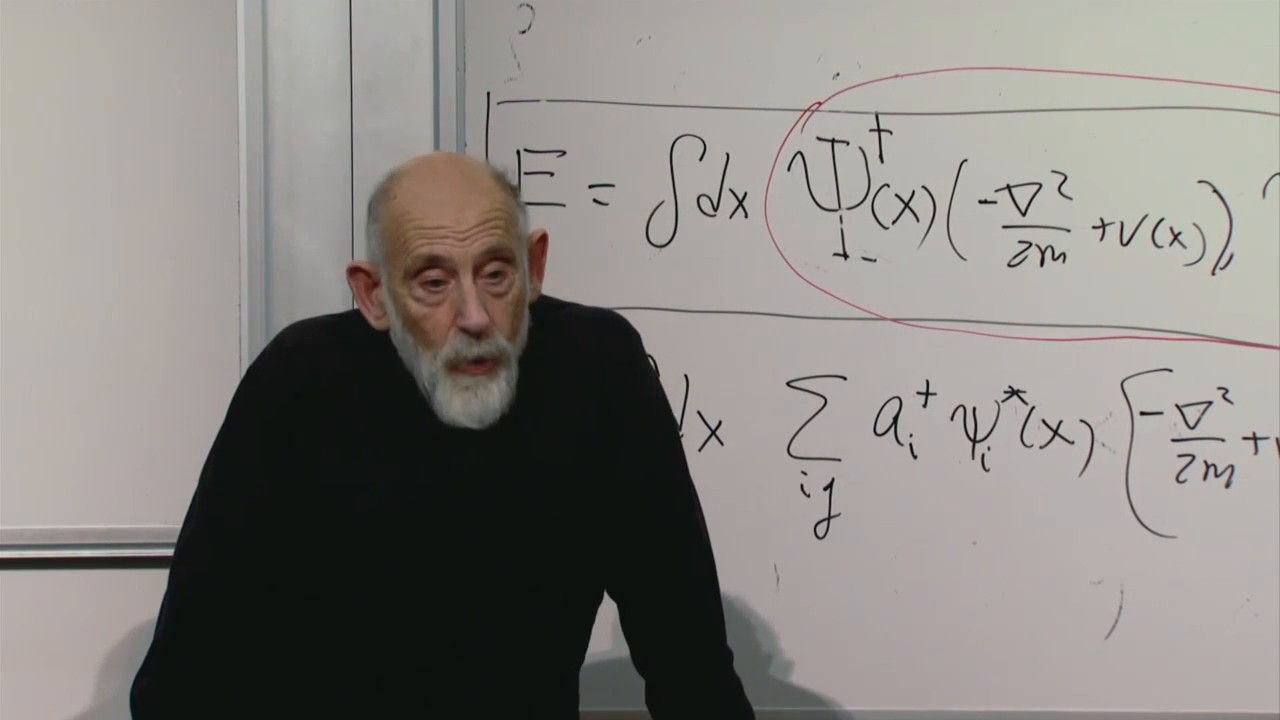
\includegraphics[width=0.94\linewidth]{lecture_07_frame_03.png}
\caption{칠판에서 강조한 장 해밀토니안과 그 아래 시작되는 모드 전개 증명. 실제 강의 화면을 증거로 남겼고, 식들~\eqref{eq:l07-field-hamiltonian}--\eqref{eq:l07-h-proof}은 전체 대수 전개를 복원한다.}
\lectureframe{01:05:34}
\end{figure}

이 유도에서는 생성 연산자를 소멸 연산자 너머로 바꾸어 놓지 않았다. 처음부터 끝까지 \(a_i^\dagger a_j\)의 순서를 유지했다. 자유롭게 옮긴 것은 \(c\)수인 파동함수와 그 고윳값뿐이다.

\section{왜 장이라고 부르는가}

\(\Psi(x)\)를 장이라 부르는 이유는 공간의 모든 점에서 정의된 연산자값 물리량이기 때문이다. 여기서 만든 에르미트 조합이나 쌍선형식은 국소 관측량이다. 밀도 \(n(x)\)와 아래에서 나올 국소 에너지 표현이 두 예다. 이 말에는 그 밖의 별도 수학적 조건이 숨어 있지 않다.

이 장은 전자기장이 아니다. 한 입자 모드와 해밀토니안 \(p^2/(2m)+V\)을 제공한 비상대론적 입자 종을 기술한다. 예를 들면 느리게 움직이는 원자, 중성자, 양성자 또는 전자다. 이 입자들은 대응하는 장의 양자이며, 그 구조적 의미에서 광자가 전자기장의 양자인 것과 같다.

\begin{classroomqa}
\lecturetimestamp{01:02:45}
\audiencequestion{다입자계에서 위 식으로 넘어오는 과정에서 장은 어디에 들어갔나요?}
\lecturerresponse{식~\eqref{eq:l07-field-expansion}에서 들어갔습니다. \(\Psi(x)\)는 각 공간점에 정의된 연산자입니다. 이어지는 유도는 그 국소 곱이 입자 밀도와 에너지 밀도를 측정함을 보여 줍니다. 위치 의존성과 연산자 성질이 함께 있다는 것이 여기서 구성하는 장의 구조입니다.}
\end{classroomqa}

\section{국소 에너지 밀도}

식~\eqref{eq:l07-field-hamiltonian}은 전체 에너지를 공간에 대한 적분으로 쓴다.
\begin{equation}
\begin{aligned}
H&=\int dx\,\mathcal H(x),\\
\mathcal H(x)
&=-\frac{1}{2m}\Psi^\dagger(x)\nabla^2\Psi(x)\\
&\quad+V(x)\Psi^\dagger(x)\Psi(x).
\end{aligned}
\label{eq:l07-hamiltonian-density}
\end{equation}
적분 안의 함수는 이 해밀토니안에 대한 자연스러운 국소 에너지 밀도다. 국소 형태는 유일하지 않다. 예를 들어 부분적분을 하면 운동 에너지 항은
\begin{equation}
\mathcal H_{\rm kin}(x)
=\frac{1}{2m}\nabla\Psi^\dagger(x)\mathbin{\cdot}\nabla\Psi(x)
\label{eq:l07-kinetic-density}
\end{equation}
로 바뀌며, 경계항이 추가된다. 통상적인 경계 조건 아래에서는 두 표현 모두 같은 전체 해밀토니안을 준다. 강의에서 언급한 작은 모호성이 바로 이것이다.

\begin{classroomqa}
\lecturetimestamp{01:05:57}
\audiencequestion{에너지 밀도는 공간 전체에 대해 적분해야 하나요?}
\lecturerresponse{공간 전체에 대해 적분하면 총에너지를 얻습니다. 더 작은 영역에 대해 적분하면 그 영역에 귀속되는 에너지를 얻습니다. 다만 전체 적분이 같은 해밀토니안이 되도록 국소 밀도를 고를 때 생기는 통상적인 모호성은 남습니다.}
\end{classroomqa}

\begin{classroomqa}
\lecturetimestamp{01:06:25}
\audiencequestion{에너지 식의 대문자 \(N_i\)는 소문자 \(n_i\)와 어떻게 다른가요?}
\lecturerresponse{\(N_i=a_i^\dagger a_i\)는 연산자입니다. 정수 \(n_i\)는 점유수 상태에서 그 연산자가 갖는 고윳값 가운데 하나입니다. 연산자는 상태에 작용하고, 그 고윳값은 보통의 수입니다.}
\end{classroomqa}

\begin{classroomqa}
\lecturetimestamp{01:06:46}
\audiencequestion{장 해밀토니안 자체를 디랙 표기법의 브라나 켓으로 쓸 수 있나요?}
\lecturerresponse{아닙니다. 브라와 켓은 상태 벡터와 그 쌍대 벡터를 나타냅니다. 장과 해밀토니안은 그 상태들에 작용하는 연산자입니다. \(\langle\Phi|H|\Phi\rangle\)와 같은 기댓값에는 두 종류의 대상이 모두 쓰이므로, 이를 서로 같은 것으로 취급해서는 안 됩니다.}
\end{classroomqa}

\section{한 입자를 복원하고 고전장에 다가가기}

확장된 형식론에는 보통의 한 입자 양자역학이 포함되어 있다. 포크 공간을 다음 조건을 만족하는 상태들로 제한하자.
\begin{equation}
N|\Phi\rangle=|\Phi\rangle.
\end{equation}
그 부문 안에서 장의 구성은 모든 한 입자 상태와 모든 한 입자 예측을 재현한다. 이전 이론을 대체한 것이 아니다. 입자가 없거나 둘 또는 임의의 수만큼 있는 계도 기술할 수 있는 공간 안에 이전 이론을 포함시킨 것이다.

반대쪽 극한에서는 보손이 매우 많이 점유한 모드가 고전파동처럼 근사적으로 거동할 수 있다. 적절한 결맞음 상태나 준고전 상태에서 기댓값
\begin{equation}
\Phi_{\rm cl}(x,t)=\langle\Psi(x,t)\rangle
\end{equation}
은 자유 비상대론 이론에서 다음과 같은 고전적 형태의 방정식을 따른다.
\begin{equation}
i\partial_t\Phi_{\rm cl}(x,t)
=\left(-\frac{\nabla^2}{2m}+V(x)\right)\Phi_{\rm cl}(x,t)
\label{eq:l07-classical-schrodinger}
\end{equation}
강의에서는 이 관계를 유도하지 않고 언급한다. 이것은 양자들의 집합과 파동장 사이를 잇는 다리다. 점유수가 크면 상대 요동이 억제되어 적절한 기댓값이 고전적으로 거동한다.

따라서 이 형식론은 계산상의 정리 도구인 동시에 물리적 내용도 담는다. 모든 입자 수 부문을 체계화할 뿐 아니라, 간섭과 얽힘, 양자 입자에서 고전파동이 나타나는 과정도 포착한다.

\begin{classroomqa}
\lecturetimestamp{01:10:43}
\audiencequestion{적분 안에서 생성 연산자와 소멸 연산자를 보통 수처럼 다뤄도 되는 이유는 무엇인가요?}
\lecturerresponse{두 연산자를 서로 바꾼 적은 없습니다. 보통의 모드 함수는 연산자와 가환하고, 미분은 그 함수에만 작용합니다. 소멸 연산자를 생성 연산자 너머로 옮기려면 교환자를 써야 하며, 그러면 항이 하나 추가될 수 있습니다. 증명에서는 그런 이동을 하지 않습니다.}
\end{classroomqa}

\section{디랙 표기법에 대한 짧은 설명}

혼란의 일부는 역사적인 데서 비롯된다. 한 입자 파동함수는 파동 방정식을 따르므로 겉보기에는 고전장과 비슷하지만, 동시에 확률 진폭이기도 하다. 초기 양자론은 이 두 역할을 구분한 다음, 전자기장처럼 실제로 측정 가능한 파동장이 어떻게 양자로 이루어지는지 설명해야 했다. 포크 공간과 연산자값 장은 이 겉보기 모순을 해소한다.

디랙 표기법은 이 구분을 특히 간결하게 표현한다. 켓은 벡터 공간에 속하고, 브라는 그 쌍대 공간에 속하며, 둘을 나란히 놓으면 내적이 된다. 그러면 완비성 관계
\begin{equation}
\sum_i|i\rangle\langle i|=\mathbf 1
\end{equation}
의 뜻이 거의 저절로 드러난다. 강의에서는 수학자들에게 양자역학을 가르칠 때의 일화를 들어 이를 설명한다. 수학적 내용은 이미 익숙했지만, 표기법이 일상적인 조작을 매우 투명하게 보여 주어 그 구조가 새롭게 보였다는 이야기다. 요점은 어느 한 분야에 개념이 없었다는 것이 아니다. 적절한 표기법을 쓰면 허용되는 연산을 혼동하기 어려워진다는 데 있다.

이 교훈은 여기서 중요하다. 이제 서로 구별되는 여러 연산자가 있다.
\begin{itemize}
\item \(h\)는 한 입자 파동함수에 미분 연산자로 작용한다.
\item \(a_i\)와 \(a_i^\dagger\)는 포크 공간의 점유수 상태에 작용한다.
\item \(\Psi(x)\), \(\Psi^\dagger(x)\), \(N\), \(H\)도 포크 공간에 작용한다.
\end{itemize}
식~\eqref{eq:l07-field-expansion}의 전개는 이 두 맥락을 연결하지만 하나로 합치지는 않는다.

\begin{classroomqa}
\lecturetimestamp{01:18:16}
\audiencequestion{장은 입자들의 집합을 기술하는 형식론에 불과한가요?}
\lecturerresponse{장은 형식론이지만 내용 없는 형식론은 아닙니다. 그 국소 관측량은 측정할 수 있고, 입자들은 고전적인 알갱이가 아니라 간섭과 얽힘을 나타내는 양자 입자입니다. 장 연산자는 이런 측정 가능한 집단적 성질을 정확히 부호화합니다.}
\end{classroomqa}

\section{상대론에 대한 주의와 전자기장에 관한 덧붙임}

지금까지의 구성은 비상대론적이다. 상대론적 물리에서도 운동량은 입자를 나타내는 좋은 표지이지만, 위치를 정확히 국소화하는 일은 훨씬 까다롭다. 따라서 국소 광자 수 밀도는 일반적으로 비상대론적 \(n(x)\)만큼 명료한 개념이 아니다. 에너지 밀도는 잘 정의되어 있으므로 국소 관측량으로 더 안전하다.

강의에서는 유용하지만 명시적으로 직관적인 전자기 유비를 제시한다. 전기장과 자기장을 복소 벡터로 합쳐
\begin{equation}
\mathbf F=\mathbf E+i\mathbf B,
\qquad
\mathbf F^*=\mathbf E-i\mathbf B.
\label{eq:l07-riemann-silberstein}
\end{equation}
라고 하자. 그러면
\begin{equation}
\mathbf F^*\mathbin{\cdot}\mathbf F
=\mathbf E^2+\mathbf B^2,
\label{eq:l07-em-density}
\end{equation}
이며, 이는 통상적인 단위계에서 전자기 에너지 밀도에 비례한다. 이것은 광자 확률 밀도와 문자 그대로 같은 것이 아니다. 제곱 크기가 에너지 밀도를 나타내는 간결한 장 변수로 보는 편이 낫다. 또는 비공식적으로는 광자 에너지로 가중한 광자 밀도라고 할 수 있다.

\begin{classroomqa}
\lecturetimestamp{01:19:10}
\audiencequestion{광자 밀도를 전기장 세기와 동일시할 수 있나요?}
\lecturerresponse{정성적으로만, 그리고 주의해서 그렇습니다. 상대론적 광자에 대해서는 국소 입자 수가 적절한 개념이 아닙니다. 확실하게 말할 수 있는 것은 \(E^2+B^2\)가 에너지 밀도에 비례하고, 복소 조합 \(\mathbf E+i\mathbf B\)가 맥스웰 방정식을 슈뢰딩거 방정식과 비슷한 형태로 묶어 준다는 점입니다.}
\end{classroomqa}

\begin{classroomqa}
\lecturetimestamp{01:20:09}
\audiencequestion{상대론적 입자의 위치는 문제가 되는데 운동량은 왜 정해질 수 있나요?}
\lecturerresponse{운동량은 상대론적 한 입자 표현을 깔끔하게 표시하지만, 입자 생성 및 상대론적 장 기술과 정확한 국소화는 양립하기 어렵습니다. 이 강의에서는 그 이론을 전개하지 않습니다. 여기서의 주의는 비상대론적 밀도 해석이 적용되는 범위를 표시합니다.}
\end{classroomqa}

\section{연산자 순서와 바닥 상태 상수}

연산자 순서를 함부로 바꾸어서는 안 된다. 보손 모드에서는
\begin{equation}
a_i a_i^\dagger=a_i^\dagger a_i+1.
\end{equation}
가 성립한다. 따라서 정규 순서인 \(\Psi^\dagger h\Psi\)를 반대 순서인 \((h\Psi)\Psi^\dagger\)로 바꾸거나, 이에 상응하는 적분 형태로 바꾸면 교환자 항이 추가된다. 모드 기저에서는 모드마다 양자 하나의 에너지를 더한 합이다. 이것은 바닥 상태 에너지, 즉 영점 에너지 상수이며, 연속체에서는 정칙화가 필요하다. 강의에서는 여기서 이 문제를 더 다루지 않고, 두 연산자 순서가 같지 않다는 점만 경고한다.

\begin{classroomqa}
\lecturetimestamp{01:22:04}
\audiencequestion{해밀토니언에서 \(\Psi\)와 \(\Psi^\dagger\)의 순서를 바꾸면 어떻게 될까요?}
\lecturerresponse{교환자도 포함해야 합니다. 따라서 순서를 바꾸면 같은 식이 되는 것이 아니라, 상태와 무관한 바닥 상태 기여가 더해집니다. 여기에 제시된 해밀토니언은 정규 순서로 썼습니다. \(\Psi^\dagger h\Psi\).}
\end{classroomqa}

\section{운동량으로 마무리 점검}

마지막 몇 분 동안 같은 승격 과정을 한 번 더 살펴봅니다. 입자 하나에 대해서는
\begin{equation}
\langle p\rangle_\psi
=\int dx\,\psi^*(x)\left(-i\partial_x\right)\psi(x).
\label{eq:l07-one-particle-momentum}
\end{equation}
파동함수를 장으로 바꾸면 전체 운동량 연산자는 다음과 같습니다.
\begin{equation}
P=\int dx\,\Psi^\dagger(x)\left(-i\partial_x\right)\Psi(x),
\label{eq:l07-field-momentum}
\end{equation}
또는 3차원에서는
\begin{equation}
\mathbf P=\int d^3x\,\Psi^\dagger(\mathbf x)
\left(-i\boldsymbol\nabla\right)\Psi(\mathbf x).
\end{equation}
장도 운동량을 가집니다. 충분히 강력한 레이저는 벽에 운동량을 전달해 힘을 가합니다. 양자론적 기술에서 장의 운동량은 광자들의 운동량을 모두 더한 것입니다.

식~\eqref{eq:l07-field-momentum}은 기댓값이 아니라 연산자입니다. Fock 공간 상태 \(|\Phi\rangle\)가 주어지면 다음을 계산할 수 있습니다.
\begin{equation}
\langle P\rangle_\Phi=\langle\Phi|P|\Phi\rangle.
\end{equation}
기댓값을 구하려면 연산자와 상태가 모두 필요합니다. 관측량과 그 평균을 혼동하면 이 강의에서 확립해 온 바로 그 구분이 사라집니다.

\begin{classroomqa}
\lecturetimestamp{01:26:02}
\audiencequestion{여기에 제시된 장의 운동량은 이미 평균 운동량인가요?}
\lecturerresponse{아닙니다. 이것은 관측량을 나타내는 에르미트 연산자입니다. 상태를 정한 다음 그 상태의 브라와 켓 사이에 연산자를 놓아 기댓값을 구해야 합니다. 측정값은 여전히 그 평균을 중심으로 요동할 수 있습니다.}
\end{classroomqa}

여기서 마무리하는 것이 자연스럽습니다. 입자에서 출발해 국소적인 생성장과 소멸장을 구성하고, 이를 이용해 입자 수를 세었으며, 입자 하나의 에너지와 운동량을 모두 합한 양을 장 연산자로 다시 썼습니다. 다음 단계는 표기법을 또 바꾸는 것이 아닙니다. 장 연산자로 물리적 과정을 나타내는 것입니다. 입자의 붕괴, 입자의 산란, 그리고 서로 다른 종 사이의 변환을 다룹니다.
